\chapter{Evaluation}\label{chap:6}


\section{Accuracy evaluation}

In 4436 malwares obtained, 4181 of them are to construct a decision trees. The number of each malware families is shown in Table \ref{table:trainingdata}. Then, 255 remaining malwares meta-data are kept to test experimental result the system.
\begin{table}
  \begin{center}
    \begin{tabular}{ | l | l |}
     \hline
    Malware & Number\\ \hline
    Virut & 2243\\ \hline
	IRCbot & 1169\\ \hline
	Gaobot  & 265\\ \hline
	Autorun & 195\\ \hline
	Downadup &  103\\ \hline
	Mota & 79\\ \hline
	Sality  & 66  \\ \hline
	WaledacMota & 61\\ \hline
    \end{tabular}
	\end{center}
     \caption{Training data.}
      \label{table:trainingdata}
\end{table}

In the decision tree, 255 malwares are taken to check the experimental result of system. 

 The number of each malware families is shown in Table \ref{table:testdata}
 \begin{table}
  \begin{center}
    \begin{tabular}{ | l | l |}
     \hline
    Malware & Number\\ \hline
    Virut & 200\\ \hline
	IRCbot & 100\\ \hline
	Gaobot  & 20\\ \hline
	Autorun & 10\\ \hline
	Downadup &  10\\ \hline
	Mota & 5\\ \hline
	Sality  & 5  \\ \hline
	WaledacMota & 5\\ \hline
    \end{tabular}
	\end{center}
     \caption{Test data.}
      \label{table:testdata}
\end{table}
Table \ref{table:experimentalresult} reveals that result. Some of data in axis show these total number of malware in that family, and that number is separated into groups that these malwares has been classified by the system. For example, there are four malwares in Win32/Virut family, and three of them are successfully sorted into Win32/Virut family and, while one malware is in other family. Therefore, the system recognizes the trojan agent family with 75 \% of accuracy.
\begin{table}
  \begin{center}
    \begin{tabular}{ | l | l | l | l | l | l | l | l | l | l |}
     \hline
    Malware & Virut & IRCbot& Gaobot &  Autorun & Downadup  & Mota & Sality & Waledac & Accuracy\\ \hline
    Virut & 98 & 102 & 0 & 0 & 0 & 0  & 0  & 0 & 49\%\\ \hline
    IRCbot & 5 & 95 & 0 & 0 & 0 & 0  & 0  & 0 & 95\%\\ \hline    
	Gaobot & 0 & 20 & 0 & 0 & 0 & 0  & 0  & 0 & 0\%\\ \hline
	Autorun & 10 & 10 & 0 & 0 & 0 & 0  & 0  & 0 & 0\%\\ \hline	
	Downadup & 0 & 1 & 0 & 9 & 0 & 0  & 0  & 0 & 90\%\\ \hline
	Mota  & 2 & 3 & 50 & 0 & 0 & 0  & 0  & 0 & 0\%\\ \hline
	Sality  & 1 & 1 & 50 & 0 & 1 & 2  & 0  & 0 & 40\%\\ \hline	
	Waledac & 2 & 3 & 50 & 0 & 0 & 0  & 0  & 0 & 0\% \\ \hline
    \end{tabular}
	\end{center}
     \caption{Experimental result}
    \label{table:experimentalresult}
\end{table}
The accuracy of this classification system:
\begin{equation}
Accuracy=\frac{98+95+9+2}{355}=57\%
\end{equation}

The other classification is often classify malware into benign and malicious software. The system implemented in this thesis classify malware into the malware family. Therefore, system The system is useful to help virus researcher determine the malware family that unknown malware belongs to. The malware family contains Win32/Virut, Win32/Autorun, Win32/IRCbot, Win32/Gaobot, Win32/Waledac, Win32/Downadup, Win32/Sality, W32.Mota, known as famous malware family. Virus researchers who know the family of malware can easily find out some semantic similarities between malwares and shows their inner similarity in behavior and static malware characteristics.

\section{Efficiency  of classification}
The evaluation was performed on a 2.4 HZ core i3 laptop with 4G memory, running in ubuntu 11.4. 	

To evaluate the speed of the malware classification system, 2999 malware samples were evaluate the classification efficiency of the system.
Figure \ref{fig:evaluation} show the processing time of our approach. 1606 samples required approximately 0 seconds. 1392  required 0.01 second. Only one sample required 0.02 seconds. The median time samples to perform classification for each samples is approximately 0.05 seconds.
\ref{fig:evaluation}.
\begin{figure}[h!]
\centering
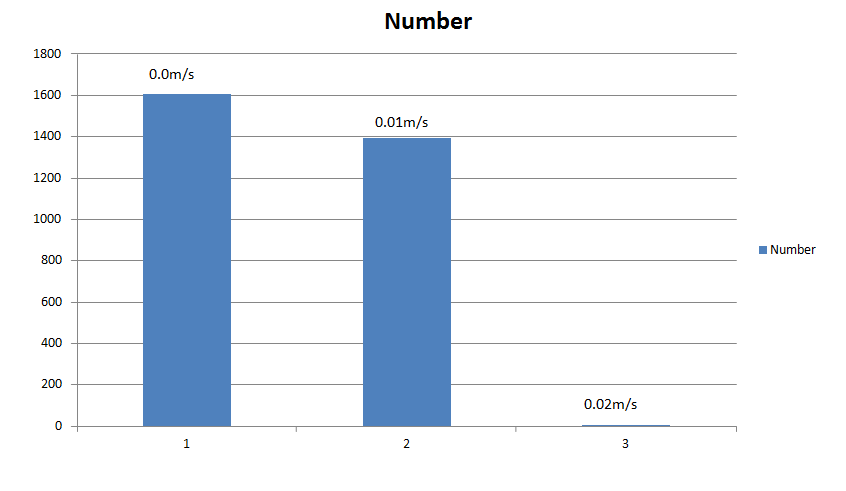
\includegraphics[width=1\textwidth]
{graph/evaluation.png}
\caption{Processing time of our approach.}
\label{fig:evaluation}
\end{figure}
The median time compared to the median time of folowgraphs appoach introduced in chapter \ref{chap:3}. The evaluation of  folowgraphs appoach was performed on a 2.4 GHz Quad Core Desktop PC with 4G of memory, running 32-bit Windows Vista Home Premium with Service Pack 1\cite{silvio}. The result was shown in figure \ref{fig:evaluation1}. The median time to perform classification was 0.25 seconds. The slowest sample that is required 5.12 seconds. Only 6 samples required more than 2 seconds. Processing time of followgraph approach was shown in figure \ref{fig:evaluation2}.
\begin{figure}[h!]
\centering
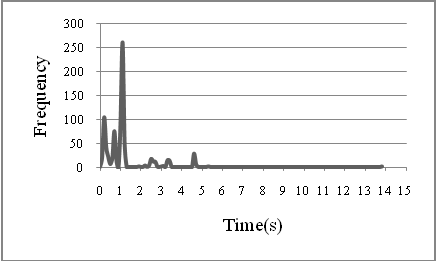
\includegraphics[width=1\textwidth]
{graph/evaluation1.png}
\caption{Processing time of followgraphs approach.}
\label{fig:evaluation1}
\end{figure}

According to the median time to perform classification, the system implemented by our approach is faster than the malware classification based on the followgraphs approach.
\section{Discussion}
\subsubsection{Accuracy evaluation}
Obviously, in experiment we obtained 4181 malware samples for constructing decision tree and 255 malware samples for evaluating system. The accuracy of our malware classification system is 57\%. However, the accuracy of Mota, Waledac, Sality samples are too low because the number of those samples is less than Virut, or IRC bot samples. There are 2243 Virut, and 1169 IRC bot samples. Otherwise, there is only 79 Mota, 61 Waledac, 66 Sality samples.

The number of Downadup samples in training data are small, but the accuracy of Downadup samples are higher than another. The reasons is Downadup binary files are different to other families so that decision tree easily identify Downadup samples.  

Moreover, all of Gaobot samples is classified into IRC bot because the Gaobot binary file is nearly similar to IRC bot.

\subsubsection{Efficiency of classification}

1606 malware samples in 2999 malware samples required approximately 0 seconds. With our approach, malware samples use meta-data to compare with each node of decision tree. In some case, malware sample 
The result of processing shows that our approach is faster than followgraphs approach. 

